% This is sigproc-sp.tex -FILE FOR V2.6SP OF ACM_PROC_ARTICLE-SP.CLS
% OCTOBER 2002
%
% It is an example file showing how to use the 'acm_proc_article-sp.cls' V2.6SP
% LaTeX2e document class file for Conference Proceedings submissions.
% ----------------------------------------------------------------------------------------------------------------
% This .tex file (and associated .cls V2.6SP) *DOES NOT* produce:
%       1) The Permission Statement
%       2) The Conference (location) Info information
%       3) The Copyright Line with ACM data
%       4) Page numbering
%
%  However, both the CopyrightYear (default to 2002) and the ACM Copyright Data
% (default to X-XXXXX-XX-X/XX/XX) can still be over-ridden by whatever the author
% inserts into the source .tex file.
% e.g.
% \CopyrightYear{2003} will cause 2003 to appear in the copyright line.
% \crdata{0-12345-67-8/90/12} will cause 0-12345-67-8/90/12 to appear in the copyright line.
%
% ---------------------------------------------------------------------------------------------------------------
% It is an example which *does* use the .bib file (from which the .bbl file
% is produced).
% REMEMBER HOWEVER: After having produced the .bbl file,
% and prior to final submission,
% you need to 'insert'  your .bbl file into your source .tex file so as to provide
% ONE 'self-contained' source file.
%
% Questions regarding SIGS should be sent to
% Adrienne Griscti ---> griscti@acm.org
%
% Questions/suggestions regarding the guidelines, .tex and .cls files, etc. to
% Gerald Murray ---> murray@acm.org
%
% For tracking purposes - this is V2.6SP - OCTOBER 2002


\documentclass[12pt]{article}

\setlength{\oddsidemargin}{0in}
\setlength{\evensidemargin}{0in}
\setlength{\topmargin}{0in}
\setlength{\headheight}{0in}
\setlength{\headsep}{0in}
\setlength{\textwidth}{6in}
\setlength{\textheight}{9in}
\setlength{\parindent}{0in} 

\usepackage{graphicx} %For jpg figure inclusion
\usepackage{times} %For typeface
\usepackage{epsfig}
\usepackage{color} %For Comments
\usepackage[all]{xy}
\usepackage{float}
\usepackage{subfigure}
\usepackage{parskip}
\usepackage{float} 

%% Elena's favorite green (thanks, Fernando!)
\definecolor{ForestGreen}{RGB}{34,139,34}
% Uncomment this if you want to show work-in-progress comments
\newcommand{\comment}[1]{{\bf \tt  {#1}}}
% Uncomment this if you don't want to show comments
%\newcommand{\comment}[1]{}
\newcommand{\jcomment}[1]{\textcolor{ForestGreen}{\comment{Jeff: {#1}}}}
\newcommand{\emcomment}[1]{\textcolor{blue}{\comment{Elena: {#1}}}}
\newcommand{\scomment}[1]{\textcolor{red}{\comment{Seth: {#1}}}}
\newcommand{\todo}[1]{\textcolor{green}{\comment{To Do: {#1}}}}

%%%%%%%%% Abbreviations of commonly used Java types %%%%%%%%%%%%
\newcommand{\AL}{{\tt ArrayList}}
\newcommand{\ALI}{{\tt ArrayListInteger}}
\newcommand{\ALIP}{{\tt ArrayList<Integer>}} % Array List with Integer parameter
\newcommand{\ALS}{{\tt ArrayListString}}
\newcommand{\ALSP}{{\tt ArrayList<String>}}
\newcommand{\ALN}{{\tt ArrayListNumber}}
\newcommand{\ALT}{{\tt ArrayList<T>}}
\newcommand{\List}{{\tt List}} %%%%%%%% \L is already defined
\newcommand{\LI}{{\tt ListInteger}}
\newcommand{\LIP}{{\tt List<Integer>}}
\newcommand{\LT}{{\tt List<T>}}
\newcommand{\ABL}{{\tt AbstractList}}
\newcommand{\ABLI}{{\tt AbstractListInteger}}
\newcommand{\Obj}{{\tt Object}}
\newcommand{\Int}{{\tt Integer}}
\newcommand{\Str}{{\tt String}}
\newcommand{\Num}{{\tt Number}}
\newcommand{\LR}{{\tt ListReader}}
\newcommand{\LRI}{{\tt ListReaderInteger}}
\newcommand{\LRIP}{{\tt ListReader<Integer>}}
\newcommand{\LRT}{{\tt ListReader<T>}}
\newcommand{\CMP}{{\tt Comparable}}
\newcommand{\CMPT}{{\tt Comparable<T>}}
\newcommand{\PQ}{{\tt PriorityQueue}}
\newcommand{\OHM}{{\tt HashMap}}
\newcommand{\OHMKV}{{\tt HashMap<K,V>}}
\newcommand{\NIS}{{\tt NarrowedIS}} %%%% Note: this is not backward-compatible with past year's macros
\newcommand{\NR}{{\tt Narrowed}}
\newcommand{\Gen}{{\tt Generic}}
\newcommand{\NISC}{{\tt NarrowedISComp}}
\newcommand{\cv}{{\tt IS-contains-v}}
\newcommand{\cvi}{{\tt containsValue}}
\newcommand{\ISPI}{{\tt IS-put-inl}}
\newcommand{\ISCVI}{{\tt IS-contains-v-inl}}
\newcommand{\IICV}{{\tt II-contains-v-inl}}

\newcommand{\T}{{\tt T}} % type parameter
\newcommand{\TB}{{\tt <T>}} % type parameter with brackets
 
%%%%%%%%% R-prefixed classes and TestInteger %%%%%%%%%%%%%%%%%%%%%%%
\newcommand{\RAL}{{\tt RArrayList}}
\newcommand{\RALI}{{\tt RArrayListInteger}}
\newcommand{\RL}{{\tt RList}}
\newcommand{\TI}{{\tt TestInteger}}

%%%%%%%%% Abbreviations of commonly used methods %%%%%%%%%%%%
\newcommand{\get}{{\tt get}}
\newcommand{\set}{{\tt set}}
\newcommand{\add}{{\tt add}}
\newcommand{\getP}{{\tt get()}}
\newcommand{\setP}{{\tt set()}}
\newcommand{\addP}{{\tt add()}}
\newcommand{\equ}{{\tt equals}}
\newcommand{\tG}{{\tt testGet}}
\newcommand{\tS}{{\tt testSet}}
\newcommand{\tA}{{\tt testAdd}}

%%%%%%%%% Abbreviations of commonly used bytecode keywords %%%%%%%%%%%%
\newcommand{\invv}{{\tt invokevirtual}}
\newcommand{\invi}{{\tt invokeinterface}}
\newcommand{\cast}{{\tt checkcast}}

%%%%%%%%%%% Groups of specializations %%%%%%%%%%%%%%%
\newcommand{\Ogroup}{{\bf O}-group}
\newcommand{\ALgroup}{{\bf AL}-group}
\newcommand{\Cgroup}{{\bf C}-group}





\begin{document}
\pagestyle{plain}
%
% --- Author Metadata here ---
%\conferenceinfo{WOODSTOCK}{'97 El Paso, Texas USA}
%\setpagenumber{50}
%\CopyrightYear{2002} % Allows default copyright year (2002) to be
%over-ridden - IF NEED BE. 
%\crdata{0-12345-67-8/90/01}  % Allows default copyright data
%(X-XXXXX-XX-X/XX/XX) to be over-ridden. 
% --- End of Author Metadata ---

\title{Improving the Interoperability between Java and Clojure}
%\subtitle{[Extended Abstract \comment{DO WE NEED THIS?}]
%\titlenote{}}
%
% You need the command \numberofauthors to handle the "boxing"
% and alignment of the authors under the title, and to add
% a section for authors number 4 through n.
%
% Up to the first three authors are aligned under the title;
% use the \alignauthor commands below to handle those names
% and affiliations. Add names, affiliations, addresses for
% additional authors as the argument to \additionalauthors;
% these will be set for you without further effort on your
% part as the last section in the body of your article BEFORE
% References or any Appendices.

\author{
Stephen Adams \\
Computer Science Discipline \\
University of Minnesota Morris\\
Morris, MN 56267\\
adams601@morris.umn.edu
}

\date{}

\maketitle
\thispagestyle{empty}

\section*{\centering Abstract}



\newpage
\setcounter{page}{1}

\section{An Introduction to Clojure}\label{sec:intro}
	Clojure is a programming language released in 2007 by Rich Hickey \cite{wiki}. Clojure is part of the Lisp family of languages. Some brief examples of Lisp-like syntax are:
	\begin{verbatim}
	(+ 2 3)
	\end{verbatim}
	Clojure uses prefix notation. To call a function you open a new list, the first thing in this list is the function name followed by the arguments. In the above case the function "+" takes in the two ints 2 and 3 and will return 5. Also note that:
	\begin{verbatim}
	(+ 2 3 4)
	\end{verbatim} 
	
	is a valid function call that returns 9. Clojure supports defining functions with a variable number of arguments. 
	
	Many of Clojure's data structures are the corresponding Java data structure; strings, characters, and numbers are just the Java implementations\cite{cloj:structs}. Clojure collections, however, are not Java collections. Clojure implements its own collections, each of these collections are denoted by different bracket types, table~\ref{coll:table} shows which literals correspond to each collection.
	
	\begin{table}[b]
	\caption{Clojure collection literals\label{coll:table}}	
	\begin{tabular}{ | l | c | }
	\hline
	Collection Type & Literal \\ \hline
	List & (1 2 3 4) \\ \hline
	Vector & ["apple" "banana" "orange"] \\ \hline
	Hashmap & \{ :address "1234 Baker St." :City Springfield :Zip 12345 \} \\ \hline
	Set & \#\{67 2 8.8 -78 \} \\
	\hline
	\end{tabular}
	\end{table}	
	Clojure code is also Clojure data types. Function calls are just lists that consist of a symbol corresponding to a function name and the arguments to that function.
	
	Clojure also includes several very powerful features for working with functions. The first allows for functions to be passed to other functions. 
	\begin{verbatim}
		(defn square [x] 
		  (* x x))
		
		(map square [1 2 3 4 5])
	\end{verbatim}
	The example above does a few things. First a new function named square is defined; square takes in one argument named x and multiplies it by itself. Then the built in Clojure function map is called. Map takes in a function and a collection and applies the function to every element of the collection. In the example the call to map will return the vector [1 4 9 16 25]. 
	
	Clojure also supports anonymous functions. 
	\begin{verbatim}
	(defn all-same [vect]
      (if 
        (empty? vect) true
        (every? (fn [x] (= (first vect) x)) (rest vect)) 
      )
    )
	\end{verbatim}
	This example function takes in a vector and checks if every element in that vector is the same. Clojure's if is a function that takes in three arguments the first is the condition which if it evaluates to true the second argument is returned otherwise the third argument is returned. The "fn" function tells the compiler that a new function is being defined within the current scope (in this case the scope is the function all-same.) In this case the anonymous function takes the first element of vect and checks if it is equal to the argument x. The outer function every? takes a function and a collection, and returns true if the function returns true for every element in the collection. Using an anonymous function here allows for the function passed to every? to use the first element in vect which would not be available to another function because it would be out of scope. First and rest just return the first element in the vector and the vector without the first element respectively.

\section{Current Java Interoperability}\label{sec:bg}
	A major feature of Clojure is that it runs on the JVM. One of the main features that Rich Hickey wanted to have when he was first designing Clojure was complete compatibility with Java and its extensive library. Since Clojure and Java code both compile down to JVM bytecode Clojure can call code written in Java. I will now briefly go over the primary methods for calling Java code.
	
	\subsection{The Dot Special form}
	The simplest way to call Java methods is with the dot(".") special form. The dot special form will first take a class member or class name then a method name then the arguments the method takes \cite{cloj:interop}. Here are a few examples of the dot in use.
	\begin{verbatim}
	(. "fred" toUpperCase)
	;;This will return "FRED".
	(.toUpperCase "fred")
	;;This also returns "FRED".
	\end{verbatim}
	The second case will actually expand into the first call and is just a shortcut for accessing fields or methods. There are a few more shortcuts to make accessing static Java methods and objects.
	
	\begin{verbatim}
	(Math/PI)
	;;Returns 3.141592653589793
	(Math/abs -2)
	;;Returns 2
	\end{verbatim}
	
	\subsection{Using Objects in Clojure}
	Static methods are only a small part of Java. Without effective ways of dealing with objects the usefulness of Java Clojure interop would be severely limited. Fortunately Clojure provides a full set of features that makes working with Java fairly easy.
	
	To construct a new object you just use the "new" special form.
	\begin{verbatim}
	(new StringBuffer "fred")
	;;Returns #<StringBuffer fred>
	\end{verbatim} 
	
	To quickly modify an object the macro doto is available. A macro is a textual transformation. Essentially a macro expands from one piece of code to another. The doto first takes a call to new, then performs the rest of the supplied arguments on that object, and finally returns the resulting object.
	\begin{verbatim}
	(doto (new StringBuffer "fred") 
	  (.setCharAt 0 \F) (.append " is a nice guy!"))
	;;Returns #<StringBuffer Fred is a nice guy!>
	\end{verbatim}
	Doto is very handy for doing sequences of set methods right after you construct an object.
	
	\subsection{Making Objects in Clojure}
	There are problems that cannot be effectively solved without creating custom classes. In particular gui programming in swing, the primary Java gui tool, is quite difficult without the ability to extend the standard swing classes. Proxy and gen-class are the two functions provided by Clojure to implement, extend, or create Java classes. 
	\subsubsection{Proxy}
	It has been said that Clojure does Java better than Java\cite{halloway:better}. I think this is most true when using proxy. It is very common when programming in Swing in particular. When creating listeners to attach to buttons or other interactive interface devices it is very common to implement many different listeners. Proxy simplifies this process by allowing you to define a single superclass with methods that will work for your interface in most circumstances; and when you need to attach a listener instead of creating an entirely new subclass use proxy to create a new class that overwrites a few methods and inherits the rest. 
	
	Proxy is a macro that takes in two vectors and then a variable number of method declarations and returns a new object. The first vector declares which Java classes the proxy object will extend and which interfaces it implements. The second vector is a list of arguments (which can be empty) to be passed to the superclass constructor. Any other arguments that are passed to proxy are method declarations\cite{cloj:interop}. 
	
	For the following proxy examples I will be using the following basic java interface:
	
	\begin{verbatim}
	public interface TestInterface {
		int square(int x);
	}
	\end{verbatim}
	This interface is in a separate interface file and is then imported into the following Clojure file.
	\begin{verbatim}
	(def test-inter 
	  (proxy [TestInterface] [] (square [x] (* x x))))
	(. test-inter square 5)
	;;Returns 25
	\end{verbatim}
	There can be more functions than just square but they have to be defined in the interface as well.
	
	\subsubsection{Gen-class}
	Proxy is limited by what is defined in a super class or Java interface, on the other hand, gen-class is designed for implementing fully featured Java classes. Gen-class consists of a set of options which are represented as key value pairs. The keys consist of Clojure keywords which are just symbols that begin with a ":." Gen-class currently supports fifteen different options. The examples below were taken from~\cite{kotka}:
	
	\begin{verbatim}
	(ns some.Example)
	(gen-class
	  :prefix method-)
	  
	(defn method-toString
	  [this]
	  "Hello, world!")
	  
	\end{verbatim}
	
	After the call to gen-class itself are the methods that are associated with the type defined by the gen-class call. This is a fairly simple example but it gives the basic idea of how gen-class works. The only option that this class uses is the prefix option. This option defines what each method that corresponds to the class must begin with. When you want to call the method on the object you would use the following code:
	
	\begin{verbatim}
	(def aClass (new some.Example))
	;;This constructs a new instance of the object
	(.toString aClass)
	;;Returns "Hello, world!" because method-toString 
	;;has the correct prefix.
	\end{verbatim}
	
	This does not make a lot of sense until you see that multiple classes can be defined in a single file.
	
	\begin{verbatim}
	(ns some.Example)
	
	(gen-class
	  :name  some.Example.classA
	  :prefix classA- )
	  
	(gen-class
	  :name some.Example.classB
	  :prefix classB- )
	  
	(defn classA-toString
	  [this]
	  "I'm an A.")
	  
    (defn classB-toString
	  [this]
	  "I'm an B.")
	\end{verbatim}
	
	When you call toString on one of these objects it will return the correct result depending on the type of the object in question. I only covered a select few of the options available to gen-class, the complete specification can be found in \cite{docs:genClass} or \cite{api:genClass}. 

		
\section{Discussion and Conclusion}\label{sec:sugg}
	In the larger scheme of the Clojure language gen-class and proxy have very limited applications. Even within the ways Clojure has of defining types that generate Java classes proxy and gen-class are in the minority. Figure~\ref{type:flow} displays a  flowchart for determining which form to use to define a new type.
	
	\begin{figure}[H]
	\begin{center}
	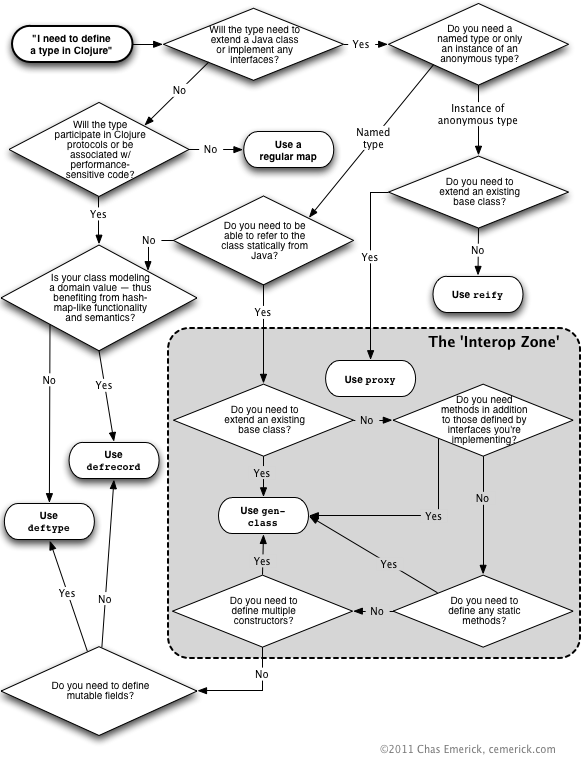
\includegraphics[scale=.55]{images/choosingtypeforms.png}
	\caption{Flowchart for choosing the correct type definition form, from \cite{choosing-types}\label{type:flow}}
	\end{center}	
	\end{figure}
	
	Gen-class and proxy are the two functions that are listed in the "interop zone." The interop zone is where Clojure's native abstractions no longer apply\cite{choosing-types}. Future directions of this project may include trying to bridge the gap between other Clojure type definitions and gen-class and proxy. This may include wrapping gen-class or proxy or extending the other Clojure type definitions so that to the end programmer all Clojure defined types look and feel like Clojure. 
	Additionally the information about Clojure-Java interop are scattered throughout many sources. A reasonable goal of this project is to collect this information in one place, this should include all of the relevant documentation, as well as examples and tutorials.
	In the forward to The Joy of Clojure\cite{joy} Steve Yegge states that it is rather surprising that a Lisp dialect has suddenly become "fashionable" again despite Clojure's lack of a killer app like Ruby has with Rails. In his contemplation on why this is he states that perhaps "the killer app for Clojure is the JVM itself. Everyone's fed up with the Java language, but understandably we don't want to abandon our investment in the Java Virtual Machine and its capabilities: the libraries, the configuration, the monitoring, and the all the other entirely valid reasons we still use it." I think that this quote simultaneously illustrates the reasons why Clojure is so compelling and why it's Java interoperability needs to be as good as possible.



%\balancecolumns

%
% The following two commands are all you need in the
% initial runs of your .tex file to
% produce the bibliography for the citations in your paper.
%\bibliographystyle{abbrv}
%\end{thebibliography}

%\bibliography{generic_types}  
% You must have a proper ".bib" file
%  and remember to run:
% latex bibtex latex latex
% to resolve all references
%
% ACM needs 'a single self-contained file'!
%
\bibliographystyle{ACM}
\bibliography{mics2012bibliography}


% That's all folks!
\end{document}

%%%%%%%%%%%%%%%%%%%%%%%%%%%%%%%%%%%%%%%%%%%%%%%%%%%%%%%%%%%%%%%%

